\subsection{Independent dosage label (ClinGen): the depletion beyond UTR length does not replicate}
gnomAD LOEUF is a population statistic, so we tested the named finding against an independent label: expert-curated ClinGen haploinsufficient genes (score 3, 420 genes), on all 43 miRNAs (13 discovery + 30 held-out). The script was committed before it was run (\texttt{clingen\_dosage}). Gates passed: the pooled CLIP universe holds 394 HI genes, and TargetScan conserved top-200 sets hold more HI genes than random UTR genes (32/5 miRNAs, $p=3.7\times10^{-6}$; pooled 307 vs 166).
\begin{table}[h]\centering\small\begin{tabular}{lcccc}\hline Pre-registered test & wins/losses & $p$ & pooled CNN / control & verdict\\\hline
C1 CNN $<$ uniform & 26/16 & $0.082$ & 158 / 205.3 & FALSIFIED \\
C2 CNN $<$ expression-matched & 28/14 & $0.022$ & 158 / 191.7 & CONFIRMED \\
C3 CNN $<$ UTR-length-matched & 24/16 & $0.134$ & 158 / 159.3 & FALSIFIED \\
\hline\end{tabular}\caption{ClinGen HI genes in CNN top-200 sets. Per-miRNA sign tests (ties excluded) and pooled counts over 43 miRNAs.}\label{tab:clingen}\end{table}
The CNN sets hold fewer HI genes than expression-matched sets (C2 confirmed; pooled ratio 0.82), but the depletion against uniform sets is not significant (C1) and it vanishes against UTR-length-matched sets (pooled ratio 0.99; C3 falsified; Figure~\ref{fig:clingen}). On this independent label, UTR length explains the depletion. The gnomAD finding therefore survives only in its weaker form (CNN candidates are less constrained than expression-matched genes); its ``beyond UTR length'' clause is supported by LOEUF but not by ClinGen. HI genes are sparse (about 4 per set), so C3 has little power; we report the disagreement rather than choosing between the labels.
\begin{figure}[h]\centering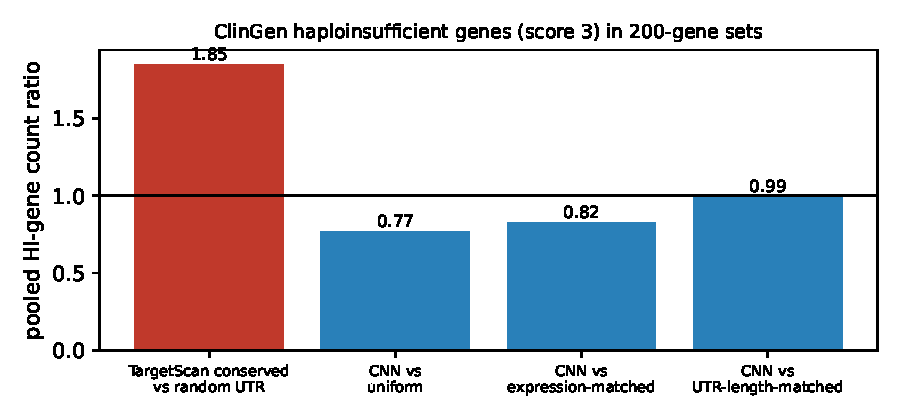
\includegraphics[width=0.62\linewidth]{figs/fig_clingen.pdf}
\caption{Pooled HI-gene count in each set divided by its control. Red: positive control.}\label{fig:clingen}\end{figure}
